\section{Week 1 Introduction}

Modern hardware does not run on single cores anymore. Execution of tasks would be too slow, it can support more than that.

\begin{figure}[H]
    \centering
    \includegraphics*[width=10cm]{res/01-stats.png}
    \caption{CPU Statistics: Jülich Supercomputing centre}
\end{figure}

\subsection*{Goals of Parallelism}

\begin{itemize}
  \item Better CPU utilization, fair division of CPU resources between tasks.
  \item more responsive programs 
  \item Divide / modularize tasks of our program 
  \item Better software division
\end{itemize}

\begin{figure}[H]
  \centering
  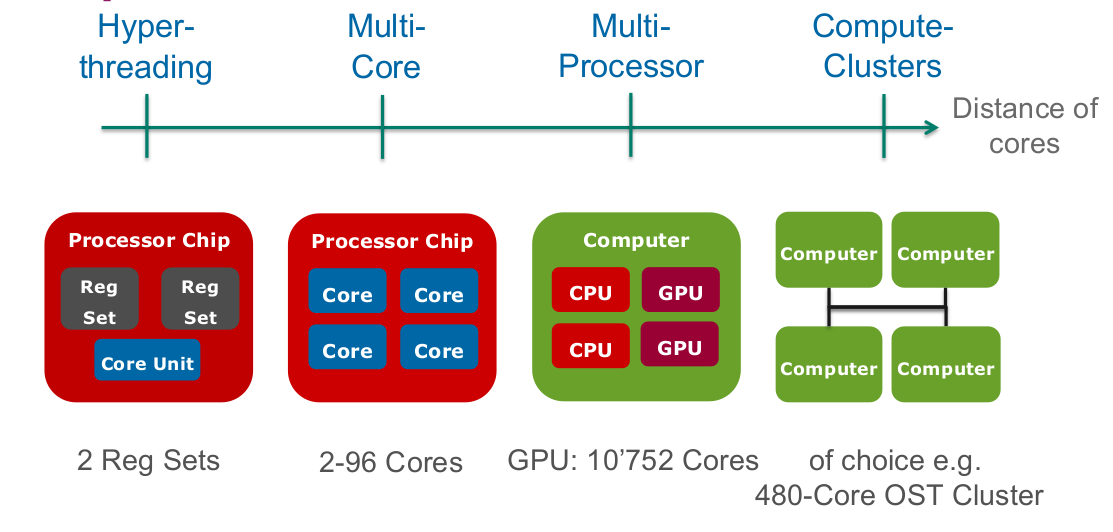
\includegraphics[width=12cm]{res/01-levels-of-parallelism}
  \caption{Levels of Parallelism}
\end{figure}

\begin{description}
  \item[Moores Law] \textit{(An observation)} The number of transistors that can be packed into a given unit of space will double about every two years.  This means the speed of a computer doubles every two years.
  Physical (atomar) limits of this law have been reached already. New ways of speeding up processors are needed.
  Modern hardware scales the amount of cores. The tasks need to be split into multiple parallel tasks to efficiently use the available cores.
  \item[Hyperthreading] Two register sets to keep two separate contexts. If one task is busy, switch to other context can happen extremely fast. Creates two logical cores from one physical core. More efficient usage of a single hardware construct, use wait time. 
  Performance increase is \emph{not} 100\% the amount of logical cores.
  \item[Parallel] Different processors act at the same time
  \item[Concurrent] Time-shared, switches between two contexts needed. One actor.
  After the end of moores law: parallelization is needed for more speedup.
  \item[Process] One program instance. Separate address space, high isolation. Context switches are slow, communication overhead.
  \begin{figure}[H]
    \centering
    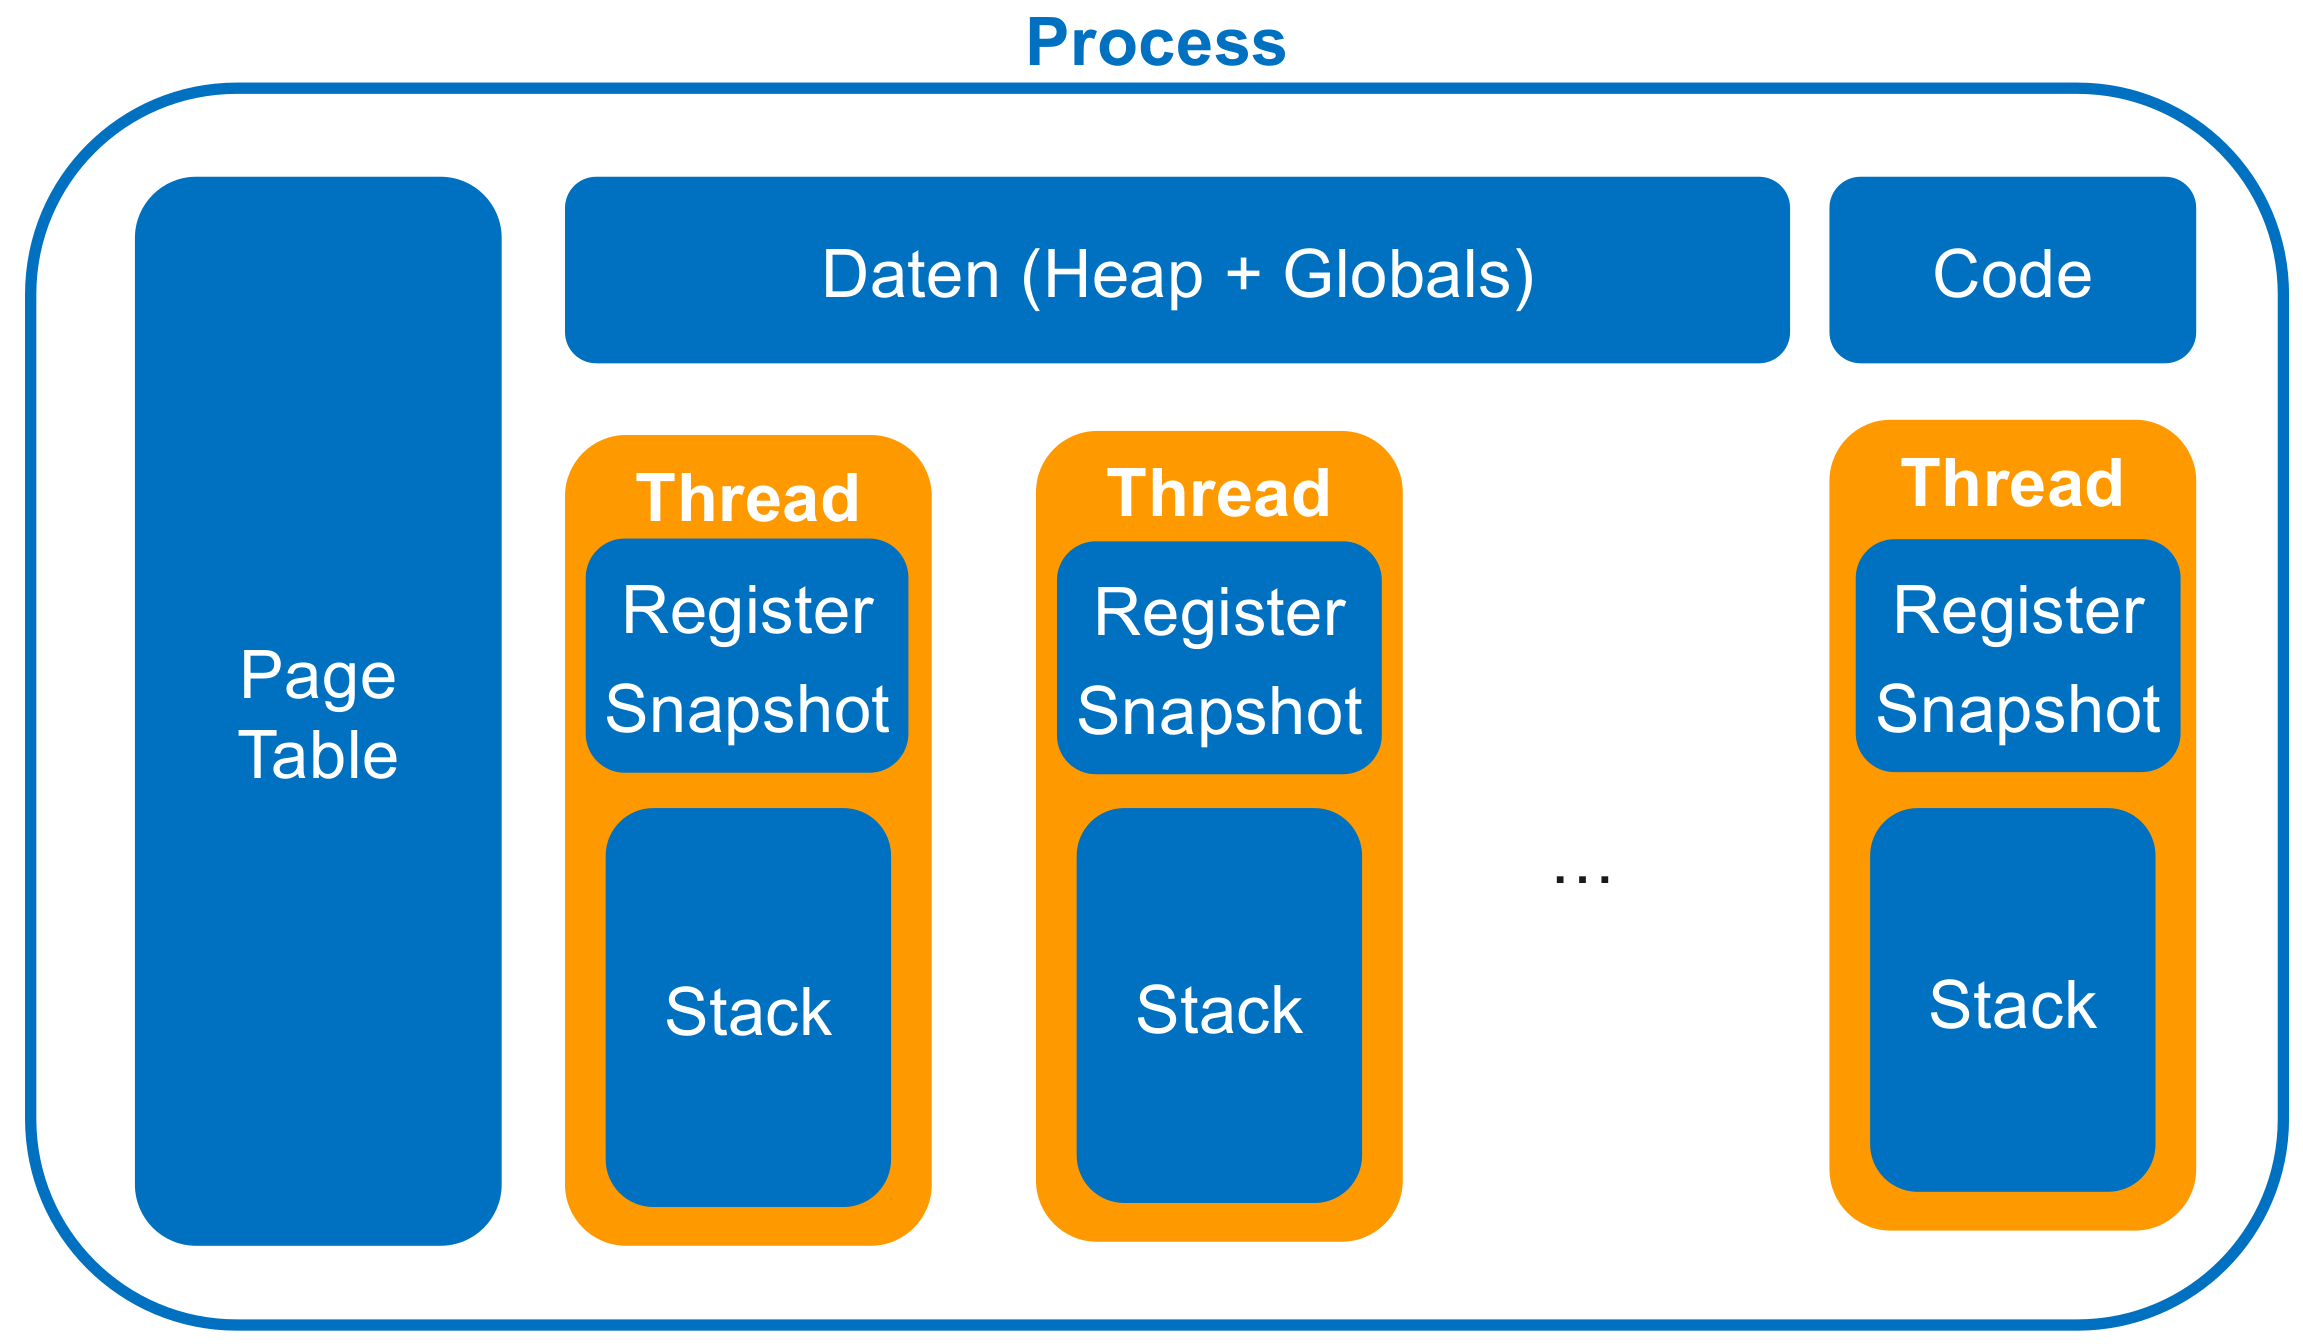
\includegraphics[width=10cm]{res/01-process.png}
    \caption{Process Internals}
  \end{figure}
  \item[Thread] Parallel sequence within a program / process. Each has their own stack and registers, but all threads inside a process share the same heap. Changes made are seen by other threads inside the process, heap access must be synchronized.
  \item[Kernel vs. user threads] 
  Only kernel-level threads let you exploit the parallelism speedup on multiple cores but are expensive in handling. User-threads (green threads, coroutines) only live within their Application. No true parallelism but concurrency. JVM always launches a kernel-level thread.

  \item[Thread Scheduling / Processor Multiplexing] This is concurrency: Interleaved execution. 
  Each processor can execute one thread at a time. Multiple Threads are managed via scheduling mechanisms.
  States: Running, ready, waiting.
  Context switches are "lightweight" but still have a performance impact.

  \item[synchronous] (cooperative) waiting for condition, thread queues itself as waiting
  \item[asynchronous] (preemptive) resources are released after a set amount of time
\end{description}

\begin{figure}[H]
  \centering
  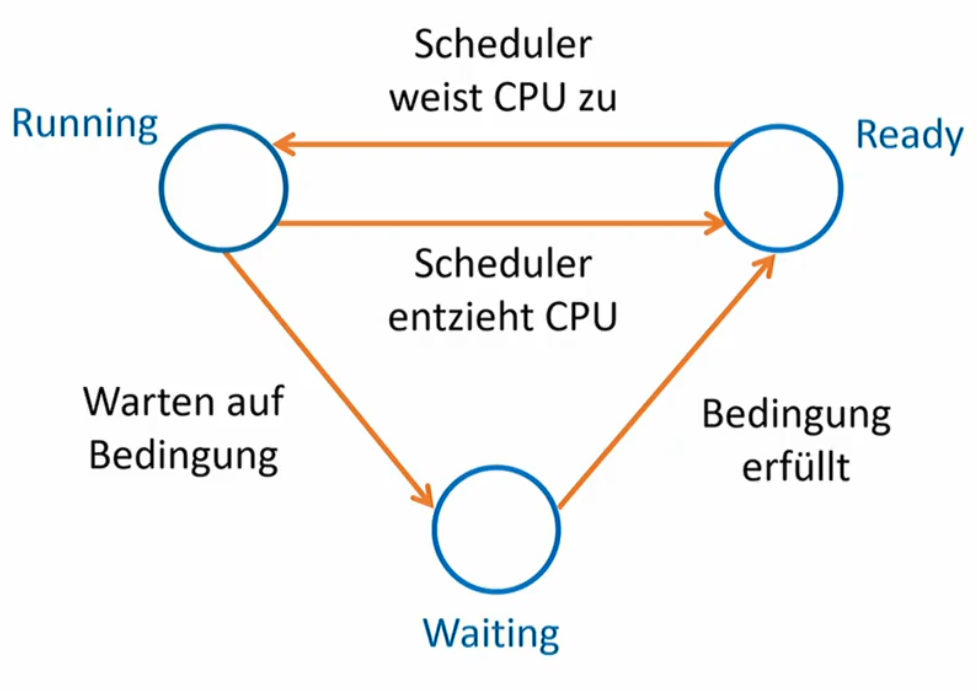
\includegraphics[width=8cm]{res/01-thread-states.png}
  \caption{Thread States}
\end{figure}

\subsection{JVM Thread Model}

\emph{intra-process communication}

The Java Virtual Machine is run as one single process. Main method is called from a startup thread created by the JVM (garbage collectors etc. start their own threads).
The JVM process runs as long as \textit{all started threads} are running. Exception: \textbf{daemon threads} are aborted at JVM end.

\texttt{Runtime.Exit()/System.exit()} end JVM abruptly.

Thread ends after exiting \texttt{run()}: either at the end of the method, on return or on an unhandled exception.

  \begin{verbatim}
    var myThread = new Thread(Runnable someAction);
    myThread.start();
  \end{verbatim}

\subsubsection{InterruptedException}
Is usually thrown by all blocking methods (\texttt{sleep, join, wait, ...}), so that an interrupt can be handled and some action performed. Best to propagate to outside of a thread. If it happens in \texttt{run()}, it needs to be caught and acted on.

\subsubsection{Non-Determinism}
No control: \textit{Threads run in any order without any precautionary rules.} \texttt{println()} in some JVMs is one synchronized (atomar) operation and will not be broken apart. This is implementation specific and not always the case. 
Only guarantee possible: statements inside one thread will always be executed in correct order.

\subsubsection{Ways to create threads}

\begin{description}
  \item[Lambda implementation] in place definition of the behaviour using lambda notation
  \begin{verbatim}
    var myThread = new Thread(() => {
      // some behaviour
    })
    myThread.start();
  \end{verbatim}

  \item[Interface Runnable] write named function that implements the interface which requires a \texttt{run()} method.
  \begin{verbatim}
    class SimpleLogic implements Runnable {
      @Override
      public void run() {
        // thread behavior
      }
    }
    var myThread = new Thread(new SimpleLogic());
    myThread.start();
  \end{verbatim}

  \item[Sub-Class of Thread] new Class with custom implementation of the run function
  \begin{verbatim}
    class SimpleThread extends Thread {
      @Override
      public void run() {
        // thread behaviour
      }
    }
    var myThread = new SimpleThread();
    myThread.start();
  \end{verbatim}
\end{description}


\subsubsection{Thread Methods}
\begin{description}
  \item[start()] executes the method \texttt{run()} of the thread object inside a newly created thread. If \texttt{run()} is called by the user, the runnable action will be run sequentially.
  \item[join()] \texttt{t2.join()} blocks t1 from running as long as t2 is still running. \texttt{currentThread().join()} creates a deadlock.
  \item[sleep()] running thread goes into waiting state until the time has passed for it to be ready again. Usage: \texttt{t1.sleep(ms)}
  \item[yield()] running thread releases the processor but will immediately be in ready state. Not really necessary in time-shared / preemptive scheduling. Use case: testing, low level performance (lock free data structures).
  \item[interrupt()] can be used for cooperative cancelling. What to do on an interrupt has to be defined by the programmer. 
  \item[currentThread()] get reference object to the currently running thread
  \item[setDaemon()] daemon threads are shut down when the JVM is stopped (Garbage Collector). Thread marked as daemon can be joined, making it "normal" again.
  \item[getId()] returns the identifier of the thread.
  \item[getName()] returns the name of the thread.
  \item[isAlive()] tests if the thread is alive.
  \item[getState()] returns the current state of the thread.
\end{description}
